\فصل{شرح مسئله}
\قسمت{علوم اعصاب نیازمند آرامش}
مطالعه فعالیت شبکه‌های عصبی برای تحقیق و بررسی کارکردهای مغز اهمیت زیادی دارد. همه بر این باوریم که مغز محمل اندیشه و تفکر است. ما کنجکاو هستیم که چگونه همکاری بین نورون‌های آن باعث می‌شود تا حافظه، کشف و پردازش صورت گیرد. شاید در نگاه اول مطالعه‌ی علوم اعصاب فقط از منظر زیست‌شناسی دارای معنا باشد اما در حقیقت مسائل علوم اعصاب چنان پیچیده و جذاب می‌نماید که توجه گستره‌ی بزرگی از علوم بنیادی از جمله فیزیک، شیمی، علوم رایانه و ... را به خود جلب کرده است. شایان ذکر است که تا کنون گرایش‌های یاد شده خدمات بزرگی را به این حیطه‌ ارائه کرده‌اند که دستاوردهای آن‌ها قابل ملاحظه است.\\

از نگاه علم فیزیک، دستگاه اعصاب مغز به مانند یک سامانه‌ی بس‌ذره‌ای است که هر ذره‌ی آن را واحدهای سلولی نورونی تشکیل می‌دهند. بی‌تردید فیزیکدانان تبحر خود را در مطالعه‌ی سامانه‌های بس‌ذره‌ای نشان داده‌اند. یک مثال بسیار آشنا برای آن‌ها مطالعه‌ی الکترون‌هاست که در میان اتم‌های فلزی نوسان می‌کنند و پدیده‌های خارق‌العاده‌ای چون رسانایی یا ابررسنایی را در کل سامانه پدیدار می‌کنند. اگر هر نورون را به مانند یک نوسانگر توصیف کنیم که میان حالت فعال [روشن] یا غیرفعال [خاموش] رفت‌وآمد می‌کند؛ آنگاه فیزیک بس‌ذره‌ای می‌تواند رفتارهای بسیاری از این سامانه را برای ما آشکار کند و چگونگی رخداد آن‌ها را با مدلسازی توضیح دهد.\\

همه‌ی دانشمندان حوزه‌ی علوم اعصاب بر این باور هستند که حافظه یا پردازش اطلاعات درون مغز به کمک «جمعیت» نورونی انجام می‌شود و هیچ «تک‌نورونی» به تنهایی نمی‌تواند این خواص را پدیدار کند. گواه آن که اگر بخشی از نورون‌های مغز را از جمعیت جدا کنیم؛ آنگاه اختلالات بسیاری در این فرآیندهای طلایی پیش می‌آید. در واقع کلید فهم دقیق این رفتارها درون برهم‌کنش‌ها نهفته است و نه مطالعه‌ی تک‌ذره و در مقیاس کوچک.\\

شاید این جملات ما را به یاد جمله‌ی معروف و تاریخی فیزیکدان بزرگ اندرسون بیاندازد. او مقاله‌ی جنجالی خود را در سال ۱۹۷۲ با عنوان تاریخی «بیشتر، متفاوت است.» منتشر کرد -شکل \ref{fig:anderson}. در واقع نقد او به جریان علمی زمان خودش آن بود که دانشمندان برای مطالعه‌ی هر پدیده‌ای آن را به تکه ‌پازل‌های کوچکتر خرد می‌کردند تا رفتار آن سامانه را توضیح دهند. او اظهار کرد که گویا سامانه‌ای که از کنار هم قرار دادن اجزای کوچک ساخته می‌شود گاه از جمع اعضا فراتر می‌رود و رفتارهایی متفاوت از خود نشان می‌دهد که درون هیچ کدام از اجزا به تنهایی قابل مطالعه نیست.\\

\begin{figure}
	\centering
	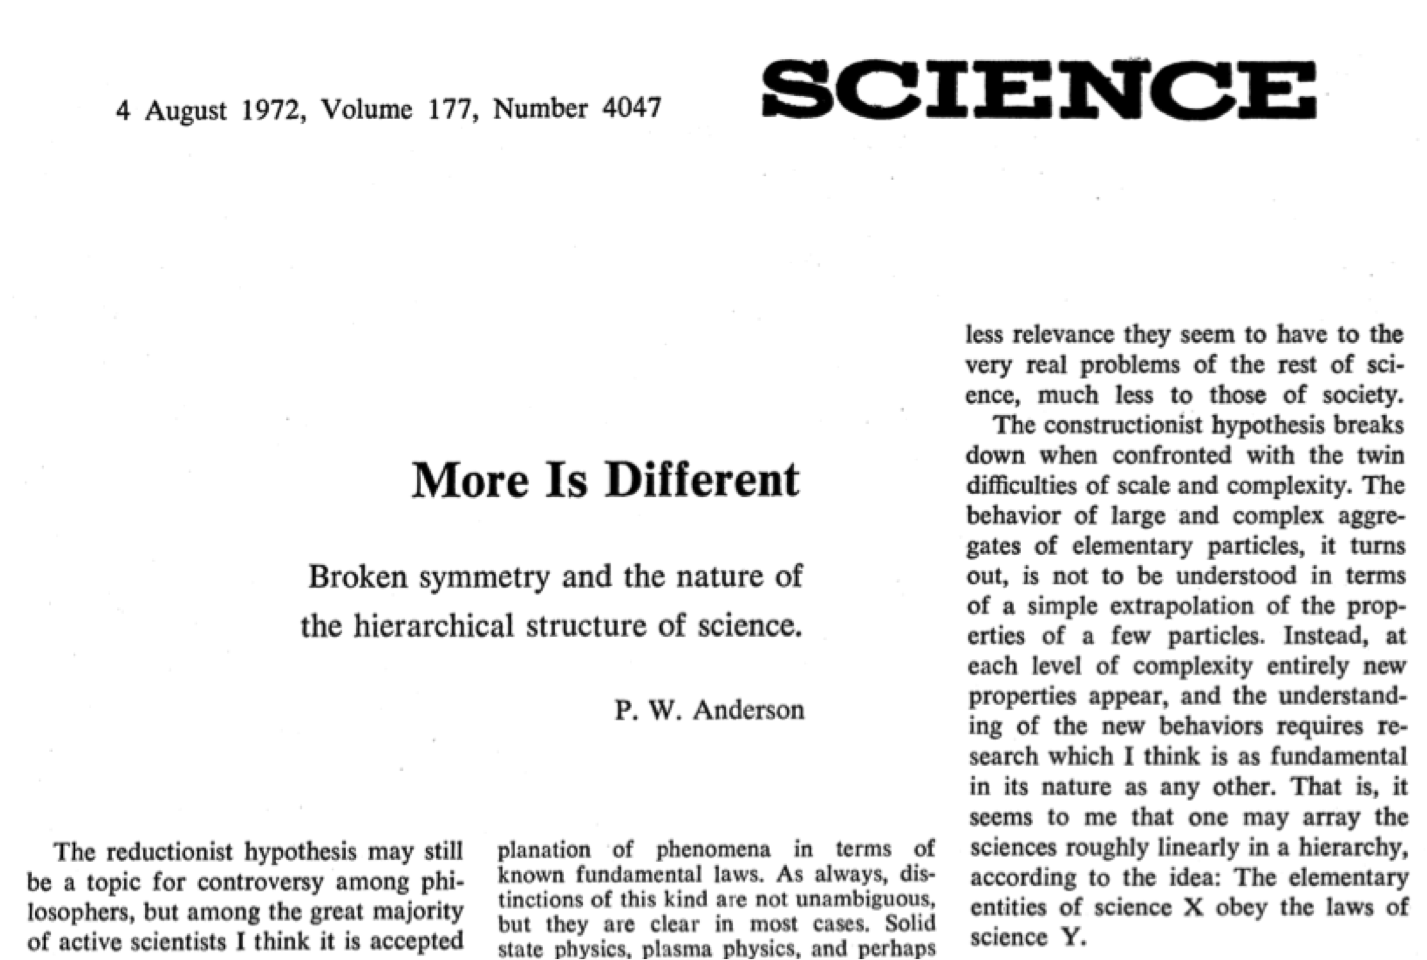
\includegraphics[width=0.5\textwidth]{../Figures/more_is_different_anderson.png}
	\caption{مقاله‌ی اندرسون در سال ۱۹۷۲ که آغازگر جهان‌بینی جدیدی در حل مسائل پیچیده بود.}
	\label{fig:anderson}
\end{figure}


او تاکید کرد که برای مطالعه‌ی برخی خواص سامانه‌های پیچیده مطالعه در مقیاس کوچک راهبردی نیست و باید کلید را در مقیاس بزرگ جستجو کرد. به عنوان مثال برای مطالعه‌ی طوفان، تشریح مولکول آب روشنگر نیست و باید همه‌ی جمعیت مولکول‌های آب را در کنار یکدیگر مطالعه کنیم. او  جهان‌بینی جدیدی را با نام «پیچیده»
\footnote{
	\lr{Complex paradigm}
}
 برای دسته‌ای از مسائل سامانه‌های بس‌ذره‌ای پیشنهاد کرد.\\
 
 اکنون که بیش از نیم‌قرن از عمر گفتمانی که او پایه‌گذاری کرد می‌گذرد؛ فیزیکدانان زیادی با جهان بینی «پیچیده» تلاش می‌کنند از علت رفتارهای جمعیتی زیادی پرده برداری کنند. یکی از معروف‌ترین شاخه‌ی این جریانات، فیزیکدانانی هستند که در حیطه‌ی علوم اعصاب فعالیت می‌کنند. آن‌ها تلاش می‌کنند با مدلسازی رفتارهای طلایی مغز همچون حافظه، خواب و ... و همچنین اختلالات و بیماری‌هایی چون آلزایمر، پارکینگسون، صرع و ... را با این جهان‌بینی توصیف کنند. کاری که در این پایان‌نامه ما انجام خواهیم داد مطالعه‌ی بیماری صرع است. یک اختلال که ناشی از فاصله گرفتن «جمعیت» نورونی از کارکرد سالم خود است.

\قسمت{کارکرد سالم}
 هر نورون‌ می‌تواند در حالت فعال [روشن] یا غیرفعال [خاموش] قرار گیرد. از آزمایش‌های بالینی انجام شده از افراد سالم دریافته‌ایم که الگوهای روشن و خاموش شدن نورون‌های مغز صورتی مشخص دارند. به این صورت که در هنگام پردازش اطلاعات دریافتی از هر ناحیه‌ی بدن تنها بخشی از مغز را به فعالیت در می‌آورد. تو گویی که هر کدام از قسمت‌های مغز وظیفه‌ی کنترل بخشی از اعضای بدن را در اختیار دارد - شکل \ref{fig:brain_anatomy}. 

\begin{figure}
	\centering
	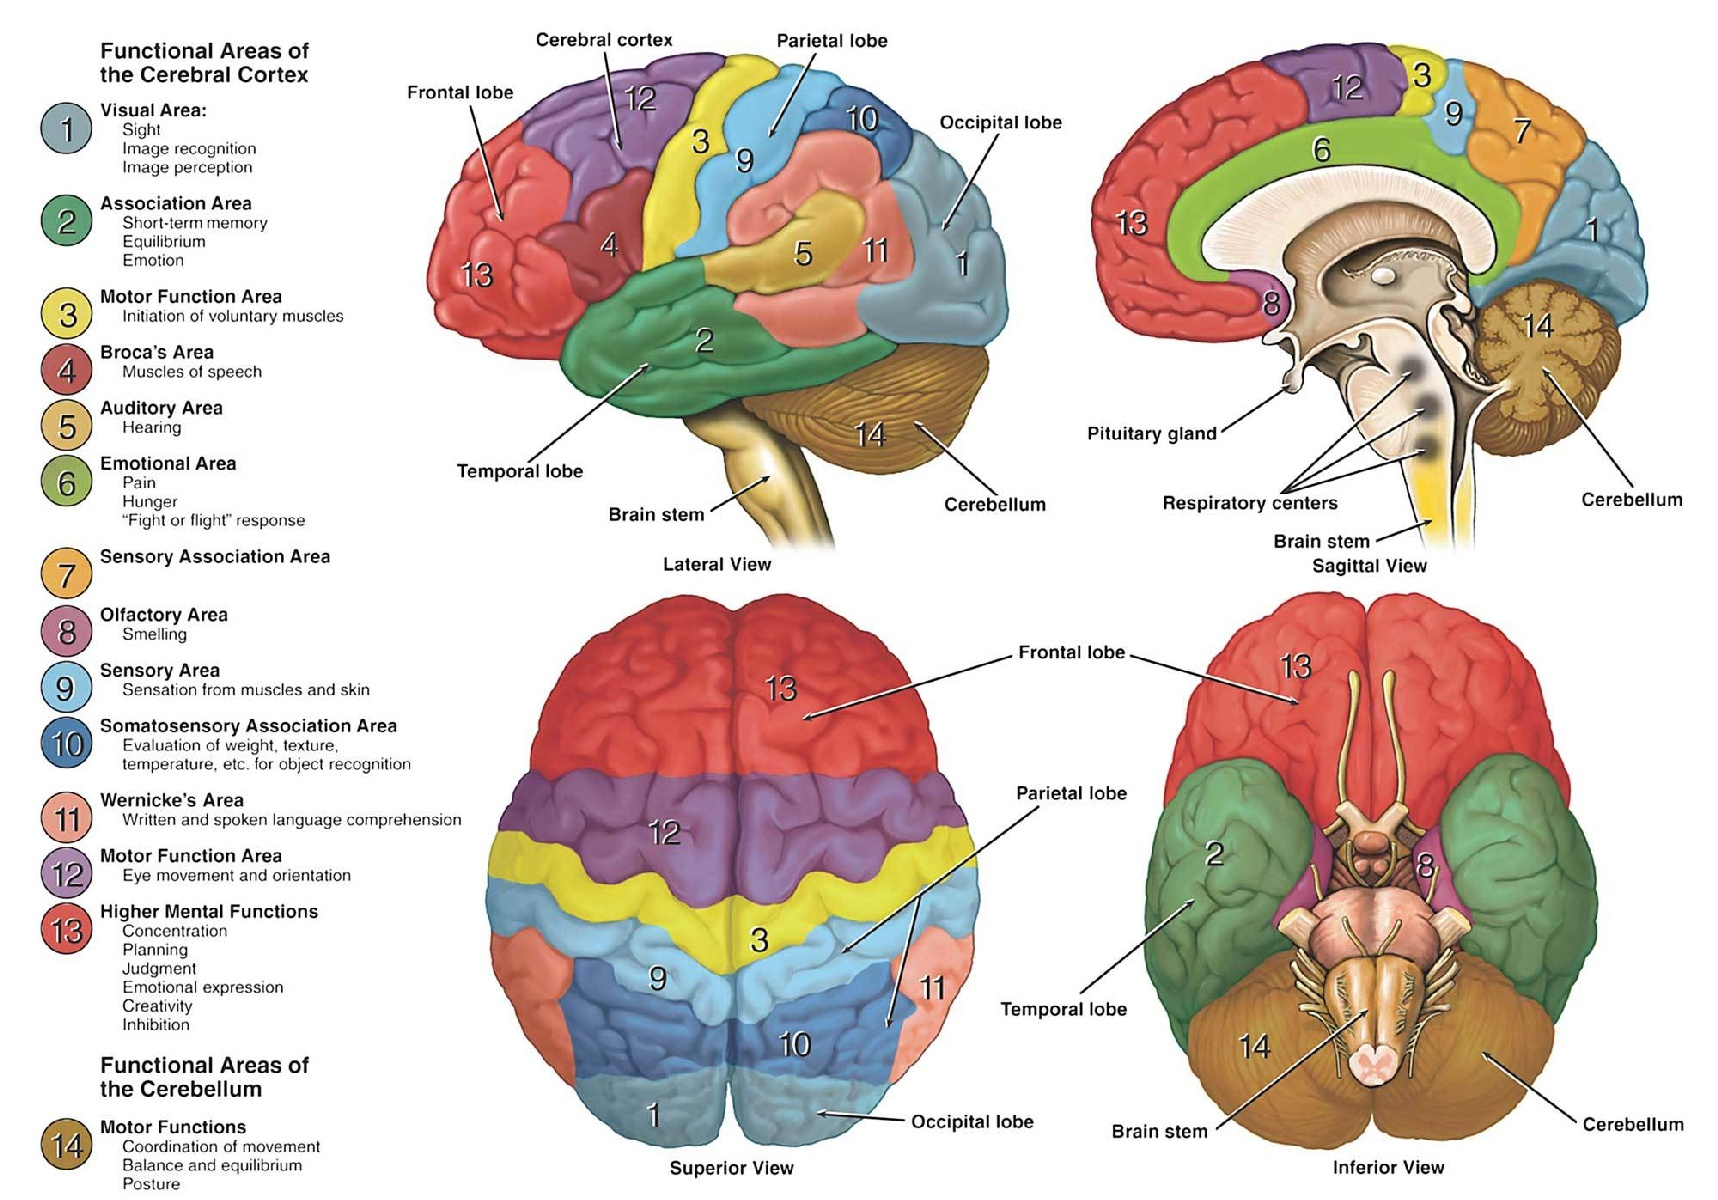
\includegraphics[width=0.5\textwidth]{../Figures/neuroanatomy_plot.jpg}
	\caption{
		تفکیک بخش‌های مختلف مغز بر حسب کنترل اعضای بدن
		\cite{penttila_2022}
	}
	\label{fig:brain_anatomy}
\end{figure}

 در حالت سالم هر کدام از ناحیه‌های مغز می‌توانند به تفکیک فعال شوند و سپس خاموش شوند. به این معنا که روشن‌وخاموش شدن یک ناحیه نباید روی ناحیه‌های همسایه به گونه‌ای مؤثر اثر بگذارد و کارکرد آن را دچار اختلال کند. در صورت بروز این اختلال فرد تمرکز خود را از کنترل یا پردازش صحیح از دست می‌دهد. به عنوان مثال سخرانان و خوانندگان پیشرفته قادر هستند تا ناحیه‌ای که مربوط به تکلم است را به تنهایی در اختیار گیرند و به صورت جداگانه به زبان بدن خود بیاندیشند. این رفتار ماهرانه اغلب در افراد مقدماتی یا دچار اختلال دیده نمی‌شود. به این ترتیب که تکلم فرد همواره همراه با الگوهای نامنظمی از تکان خوردن دست و پاست.\\
 
 بیماری صرع که در ادامه با آن آشنا خواهیم شد در واقع حالتی کاملا مختل از مغز را ناشی می‌شود که تمام ناحیه‌های مغز همدیگر را به گونه‌ای خاص مختل می‌کنند که امکان دارد فرد دارای این بیماری هشیاری خودش را کاملا از دست بدهد.

\قسمت{صرع}
شاخص‌ترین علامت بیماری صرع تشنج‌های مداوم است. گاه این تشنج‌ها در افراد بسیار خفیف و آهسته است و گاه در برخی بیماران دیگر بسیار ناگهانی و شدید اتفاق می‌افتد که می‌تواند بیمار را کاملا از هشیاری ببرد.\\

بیماری صرع یک اختلال در کارکرد جمعیت نورونی است. هم اکنون شواهدی وجود دارد که نشان می‌دهد این تشنج‌ها همراه با الگویی خاص از خاموش‌وروشن شدن جمعیت‌های نورونی همراه است. 

در زمان حمله‌ی تشنج دیده می‌شود که نورون‌های درگیر شده همگی با یکدیگر خاموش‌وروشن می‌شوند که تو گویی با یک دیگر هم‌ضربان یا \textbf{«هم‌گام»} شده‌اند. گاه این هم‌گامی فقط در یک ناحیه‌ای خاص از مغز اتفاق می‌افتد و فقط عملکرد آن ناحیه را متاثر می‌کند و گاه به ناحیه‌ای گسترده از مغز سرایت می‌کند و عملکردهای مختلف بدن را مختل می‌کند.\\

\begin{figure}
	\centering
	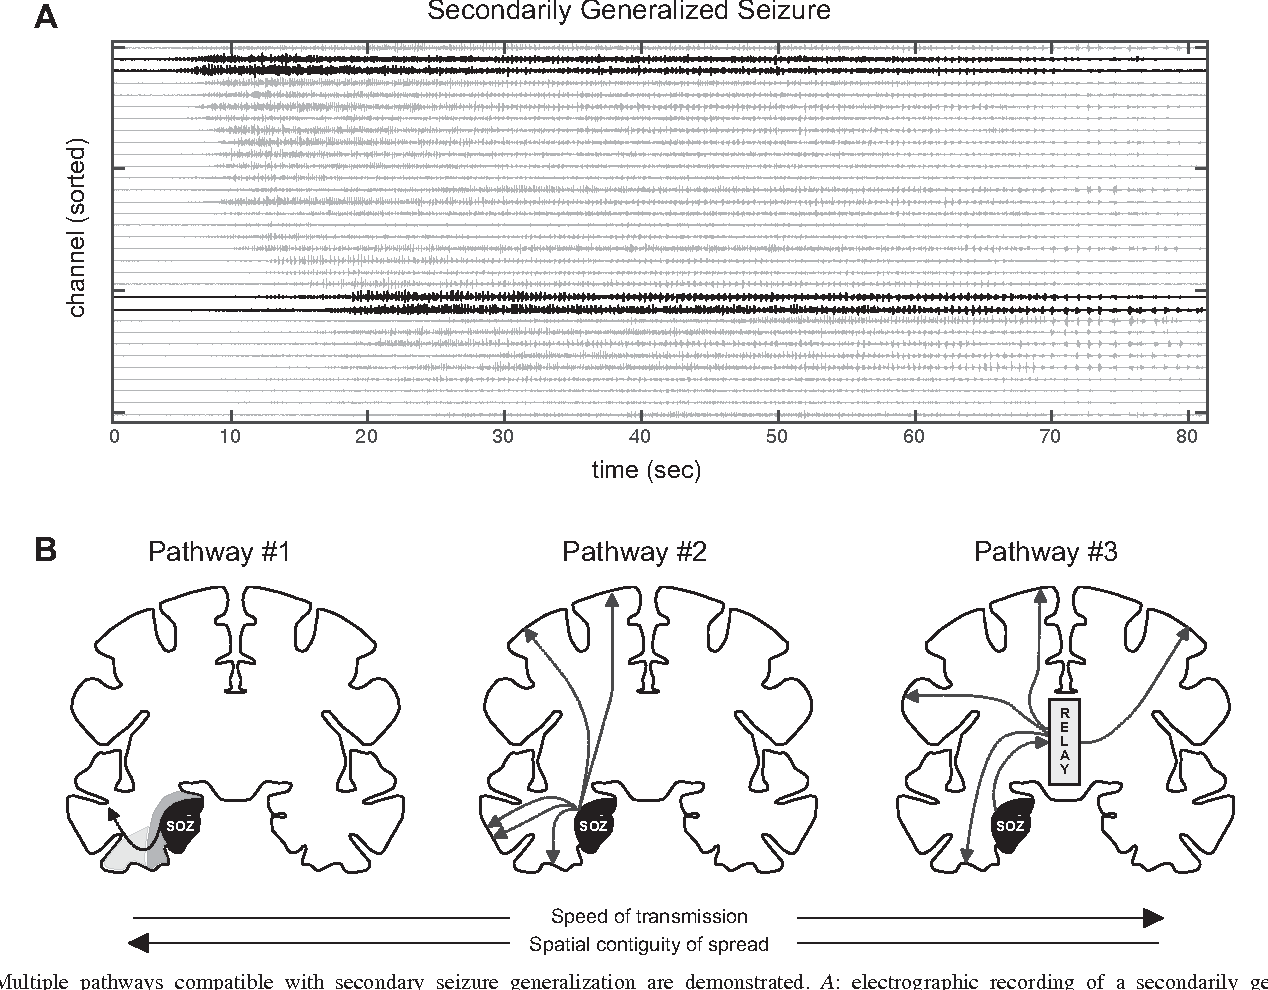
\includegraphics[width=\textwidth]{../Figures/generalized_seizure.png}
	\caption{
		سرایت هم‌گامی از کانون آن به ناحیه‌های همسایه 
		\cite{Tomlinson2017SecondaryGO}
		محور عمودی در شکل بالا نمایش دهنده‌ی شمارنده‌های گیرنده‌هایی است که سیگنال‌های دریافتی از ناحیه‌های مختلف مغز را ضبط کرده‌اند. در این شکل به وضوح می‌بینیم که پس گذشت ۱۰ ثانیه از شروع فعالیت کانون صرع، بقیه بقیه نواحی هم شروع به تشدید می‌کند و پس از گذشت ۸۰ ثانیه حمله‌ی صرع متوقف می‌شود.
	}
\end{figure}

مثلا در صورتی که کانون صرع در لوب آهیانه‌ای 
\footnote{
	\lr{Parietal Lobe}
}
باشد احتمالا منجر به اختلال در سیستم حرکتی ولرزش ماهیچه‌ها می شود، یا در لوب پس سری
\footnote{
	\lr{Occipital Lobe}
}
 و گیج گاهی
\footnote{
	\lr{Temporal Lobe}
}
  باعث اختلال در پردازش اطلاعات حسی و در لوب پیشانی
\footnote{
	\lr{Frontal Lobe}
}
   منجر به ازدست رفتن توجه و هوشیاری می‌شود.

\قسمت{لزوم شبیه‌سازی}
آیا در میان تمام میلیاردها نورون‌های مغز، نورون‌هایی که کانون صرع می‌شوند ژنتیک خاصی دارند؟ شبکه‌ی اتصال حقیقی نورون‌ها به چگونه است؟ بی‌تردید دستیابی به تمام جزییات مغز برای ما میسّر نیست اما در صورت جمع‌آوری همه‌ی این اطلاعات هم پردازش و فهمیدن آن‌ها کاری بس دشوار است. به همین علت به فراصت می‌افتیم تا اطلاعات مسئله را گزینشی‌تر بررسی کنیم و تا جایی که امکان دارد مسئله را ساده کنیم.\\

به همین دلیل به سراغ مدلسازی و آزمایش «جعبه سیاه» می‌رویم. اگر مسئله‌ی ما دشوار است تلاش می‌کنیم که با پیشنهاد مدل ساده‌ آنچه درون سامانه اتفاق می‌افتد را حدس بزنیم. سپس به سامانه‌ی شبیه‌سازی شده به آن به عنوان یک \textbf{«جعبه‌ی سیاه»} نگاه می‌کنیم (شکل 
\ref{fig:black_box})
 و بررسی می‌کنیم که چنان که انتظار می‌رود آیا توانسته‌ایم رابطه‌ی بین ورودی‌ها و خروجی‌های ثبت شده‌ی سامانه‌ی حقیقی را بازتولید کنیم یا خیر.\\

\begin{figure}
	\centering
	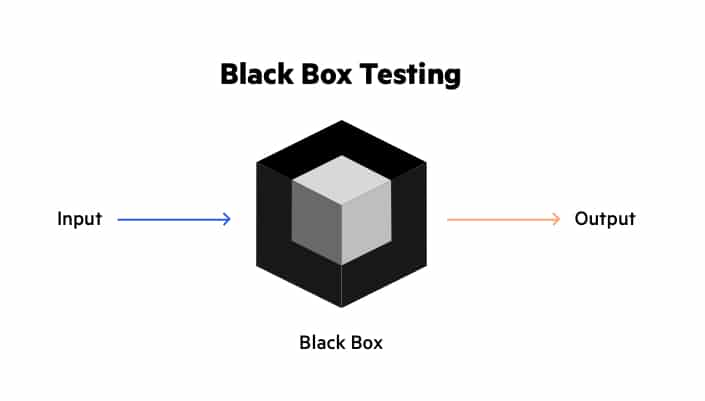
\includegraphics[width=\textwidth]{../Figures/Black_box_test.jpg}
	\caption{
		آزمایش جعبه‌ی سیاه - در این آزمایش بررسی می‌شود که آیا مدل یا برنامه‌ی ارائه شده توانسته است که با توجه به ورودی‌ها خروجی‌های مورد انتظار را بازتولید کند یا خیر.}
	\label{fig:black_box}
\end{figure}

  کاری که در این پژوهش انجام خواهیم داد تلاشی است برای پیشنهاد دادن یک مدل برای این جعبه‌ی سیاه که رفتار نسبتا مشابهی را میان ورودی و خروجی‌های این جعبه سیاه شبیه‌سازی می‌کند. همچنین به کمک بررسی دقیق‌تر این مدل تلاش می‌کنیم تا نقطه‌ی تقریبی گذرفاز سامانه را از فاز ناهم‌گام به هم‌گام پیدا کنیم.

\قسمت{مسئله‌ات را به من بده!}
مدل‌های زیادی برای شبکه‌های عصبی ارائه شده است که توانایی تولید هم‌گامی نورون‌ها را در آن‌ها می‌توانیم جستجو کنیم. یکی از این مدل‌ها که در تمام فصول شبیه‌سازی از آغاز تا کنون از آن بهره برده شده است؛ مدل انباشت و شلیک است\cite{brunel2007quantitative}. 

جستار خود را این گونه پیش می‌بریم:
\begin{enumerate}[(a)]
	\item
	ابتدا مدل پیشنهادی نویسندگان \cite{PhysRevLett.105.158104} را بازتولید می‌کنیم و تلاش می‌کنیم تا نتایج آن‌ها را دوباره بدست آوریم. بنظر می‌آید تمام کمیت‌های مهم را اندازه‌گیری نکرده‌اند. پس جوانب دیگر مسئله را هم بررسی خواهیم کرد. [به فصل 
	\nameref{chap:integrate_and_fire}
	نگاه کنید.
	]
	\item 
	«آیا این رفتار همگامی برای مدل‌های نورونی دیگر نیز اتفاق خواهد افتاد؟ یا فقط با این مدل این رفتار را مشاهده خواهیم کرد؟» پس مدل نورونی خود را عوض می‌کنیم تا پاسخ این پرسش را دریابیم. مدل پیشنهادی و جایگزین ما «چرخنده» است. [به فصل 
	\nameref{chap:rotational}
	نگاه کنید.
	]
	\item 
	تلاش کنیم تا مکان تغییر فاز به همگامی را با مدل‌های تحلیلی بدست آوریم. این کار برای مدل انباشت‌وشلیک در این مقاله 
	\cite{brunel2000dynamics}
	انجام شده است اما آیا می‌توانیم برای مدل‌های نورونی دیگر نیز آن را محاسبه کنیم؟ [به فصل 
	\nameref{chap:analytics}
	نگاه کنید.
	]
\end{enumerate}
